%%%%%%%%%%%%%%%%%%%%%%%%%%%%%%%%%%%%%%%%%%%%%%%%%%%%%%%%%%%%%%%%%%%%%%%%%%%%%%%%
%2345678901234567890123456789012345678901234567890123456789012345678901234567890
%        1         2         3         4         5         6         7         8

%\documentclass[journal,transmag]{IEEEtran}% Comment this line out if you need a4paper

\documentclass[10pt, conference]{ieeeconf}      % Use this line for a4 paper

\IEEEoverridecommandlockouts                              % This command is only needed if 
                                                          % you want to use the \thanks command

%\overrideIEEEmargins                                      % Needed to meet printer requirements.

% See the \addtolength command later in the file to balance the column lengths
% on the last page of the document

% The following packages can be found on http:\\www.ctan.org
%\usepackage{graphics} % for pdf, bitmapped graphics files
%\usepackage{epsfig} % for postscript graphics files
%\usepackage{mathptmx} % assumes new font selection scheme installed
%\usepackage{times} % assumes new font selection scheme installed
%\usepackage{amsmath} % assumes amsmath package installed
%\usepackage{amssymb}  % assumes amsmath package installed

\newtheorem{theorem}{Theorem}[section]
\newtheorem{lemma}[theorem]{Lemma}
\newtheorem{proposition}[theorem]{Proposition}
\newtheorem{corollary}[theorem]{Corollary}
\usepackage[ruled,vlined]{algorithm2e}
\usepackage{url}
\newenvironment{definition}[1][Definition]{\begin{trivlist}
\item[\hskip \labelsep {\bfseries #1}]}{\end{trivlist}}

\newcommand{\qed}{\nobreak \ifvmode \relax \else
      \ifdim\lastskip<1.5em \hskip-\lastskip
      \hskip1.5em plus0em minus0.5em \fi \nobreak
      \vrule height0.75em width0.5em depth0.25em\fi}

\def\lc{\left\lfloor}   
\def\rc{\right\rfloor}

\usepackage{amsmath,amssymb}

\usepackage{tabularx}
\usepackage{tikz,hyperref,graphicx,units}
\usepackage{subfigure}
\usepackage{benktools}
\usepackage{bbm}
\renewcommand{\baselinestretch}{.5}

\usepackage{caption}
\usepackage{epstopdf}
\renewcommand{\captionfont}{\footnotesize}
\usepackage{sidecap,wrapfig}
\usepackage[ruled,vlined]{algorithm2e}
\DeclareMathOperator*{\argmin}{arg\,min}
\DeclareMathOperator*{\argmax}{arg\,max}
\newcommand{\abs}[1]{\lvert#1\rvert} 
\newcommand{\norm}[1]{\lVert#1\rVert}
%\newcommand{\suchthat}{\mid}
\newcommand{\suchthat}{\ \big|\ }
\newcommand{\ba}{\mathbf{a}}
\newcommand{\bb}{\mathbf{b}}
\newcommand{\bc}{\mathbf{c}}
\newcommand{\bd}{\mathbf{d}}
\newcommand{\bg}{\mathbf{g}}
\newcommand{\bj}{\mathbf{j}}
\newcommand{\bn}{\mathbf{n}}
\newcommand{\bp}{\mathbf{p}}
\newcommand{\bw}{\mathbf{w}}
\newcommand{\bt}{\mathbf{t}}
\newcommand{\bu}{\mathbf{u}}
\newcommand{\by}{\mathbf{y}}
\newcommand{\bx}{\mathbf{x}}
\newcommand{\bz}{\mathbf{z}}
\newcommand{\bbf}{\mathbf{f}}
\newcommand{\bzero}{\mathbf{0}}
\newcommand{\bG}{\mathbf{G}}
\newcommand{\bA}{\mathbf{A}}
\newcommand{\bW}{\mathbf{W}}
\newcommand{\bX}{\mathbf{X}}
\newcommand{\mX}{\mathcal{X}}
\newcommand{\mD}{\mathcal{D}}
\newcommand{\mG}{\mathcal{G}}
\newcommand{\mN}{\mathcal{N}}
\newcommand{\mW}{\mathcal{W}}
\newcommand{\mF}{\mathcal{F}}
\newcommand{\bZ}{\mathbf{Z}}
\newcommand{\mR}{\mathcal{R}}

\newcommand{\bfc}{W}
\newcommand{\Qinf}{Q_{\infty}}
\newcommand{\st}[1]{_\text{#1}}
\newcommand{\rres}{r\st{res}}
\newcommand{\pos}[1]{(#1)^+}
\newcommand{\depth}{\operatorname{depth}}
\newcommand{\dist}{\operatorname{dist}}
\newcommand{\convhull}{\operatorname{ConvexHull}}
\newcommand{\minksum}{\operatorname{MinkowskiSum}}

\newcommand{\specialcell}[2][c]{ \begin{tabular}[#1]{@{}c@{}}#2\end{tabular}}
\newcommand{\acro}{SHIV}
\newcommand\independent{\protect\mathpalette{\protect\independenT}{\perp}}
\def\independenT#1#2{\mathrel{\rlap{$#1#2$}\mkern2mu{#1#2}}}

\newcolumntype{L}[1]{>{\RaggedRight\hspace{0pt}}p{#1}}
\newcolumntype{R}[1]{>{\RaggedLeft\hspace{0pt}}p{#1}}


\newboolean{include-notes}
\setboolean{include-notes}{true}
\newcommand{\adnote}[1]{\ifthenelse{ \boolean{include-notes}}%
 {\textcolor{blue}{\textbf{AD: #1}}}{}}
 
 \newcommand{\fpnote}[1]{\ifthenelse{ \boolean{include-notes}}%
 {\textcolor{blue}{\textbf{FP: #1}}}{}}
 
  \newcommand{\mlnote}[1]{\ifthenelse{ \boolean{include-notes}}%
 {\textcolor{purple}{\textbf{ML: #1}}}{}}

\renewcommand{\baselinestretch}{.95}
\usepackage{times}
\usepackage{microtype}
%\title{Iterative Imitation Learning with Reduced Human Supervision [v11]}
%\title{SHIV:  Reducing Human Supervision for Robot Active Learning [v11]}

\title{A Gambler's DAgger: Reducing Supervisor Burden in Online Learning From Demonstration Learning  Through Hierarchical Supervisors}



\author{Michael Laskey$^1$, Jonathan Lee$^1$, Caleb Chuck$^1$, David Gealy$^1$,...,Florian T. Pokorny,\\
 Anca D. Dragan$^1$, and Ken Goldberg$^{1,2}$% <-this % stops a space
\thanks{$^1$ Department of Electrical Engineering and Computer Sciences; {\small \{mdlaskey,iamwesleyhsieh,ftpokorny,anca\}@berkeley.edu, \small staszass@rose-hulman.edu} }%
\thanks{$^2$ Department of Industrial Engineering and Operations Research; {\small goldberg@berkeley.edu}}%
\thanks{$^{1-2}$ University of California, Berkeley;  Berkeley, CA 94720, USA}%
}
\begin{document}



\maketitle
\thispagestyle{empty}
\pagestyle{empty}


%%%%%%%%%%%%%%%%%%%%%%%%%%%%%%%%%%%%%%%%%%%%%%%%%%%%%%%%%%%%%%%%%%%%%%%%%%%%%%%%

\begin{abstract}
Online learning from demonstration algorithms such as
DAgger can learn policies for problems where the system dynamics and
the cost function are unknown. However they impose a
burden on supervisors to respond to queries each time the robot
encounters new states while executing its current best policy.  Traditionally there has only been one supervisor and it is deemed expert. However, an expert supervisor might not be needed for a large portion of the state space, which could be handled by less-skilled supervisors. We present the Gambler's DAgger, which instead of only using an expert supervisors presents a hierarchical supervisor model, that first leverages cheaper supervisors, such as analytical methods on approximate dynamics or crowdsourced Amazon Mechanical Turk workers to train the policy. Then only consults an expert supervisor for harder to learn states. We demonstrate this approach in training a visuomotor deep network policy for 2D grasping in clutter on a 4-DOF Zymark Robot. We were able to reduce the number of queries to the final expert supervisor by $X$ and manage to collect $X$K examples by leveraging the hierarchical supervisor model. 
 \end{abstract}


%%%%%%%%%%%%%%%%%%%%%%%%%%%%%%%%%%%%%%%%%%%%%%%%%%%%%%%%%%%%%%%%%%%%%%%%%%%%%%%%

\section{Introduction} 
In model-free robot Learning from Demonstration (LfD), a robot learns to perform a task, such as driving or grasping an object in a cluttered environment, from examples provided by a  supervisor, usually a human.  In such problems, the robot does not have access to either the cost function that it should optimize, nor the dynamics model. The former  when it is difficult to specify how to trade-off various aspects that matter, like a car trying to drive on the road with other cars~\cite{abbeel2004apprenticeship}.  The latter occurs when either the system or the interaction with the world is difficult to characterize, like when a robot is trying to grasp an object in clutter and does not have an accurate model of the object dynamics. 

Rather than explicitly learning the cost function as in Inverse Reinforcement Learning and the dynamics model, and then using optimization to produce a policy for the task, in model-free LfD the robot learns a policy directly from supervisor examples, mapping states to controls~\cite{argall2009survey}. Learning from demonstration has been used successfully in recent year for a large number of robotic tasks, including helicopter maneuvering~\cite{abbeel2007application}, car parking~\cite{abbeel2008apprenticeship},  and robot surgery~\cite{van2010superhuman}. 

 \begin{figure}
\includegraphics[width=0.5\textwidth]{f_figs/teaser.pdf}
\caption{Typical Initial States for our grasping in clutter task with a Zymark Robot. Red shapes indicate the clutter objects and the yellow circle indicates the goal object. The robot learns from raw image date to push the shapes and reach the yellow circle through our algorithm A Gambler's DAgger. The inscribed circle in the workspace prevents the robot from learning the trivial solution of simply pushing the red objects off the table.}
\vspace*{-20pt}
\label{fig:teaser}
\end{figure}


LfD algorithms can be categorized as offline, where the robot only observes demonstrations, or online, where the robot interacts with the world and receives feedback from the supervisor.
In offline LfD, the robot learns the policy based on a batch of examples, and then executes it to achieve the task.  During execution, a small control error can accumulate, leading the robot away from the region of the state space where it was given examples, leading to unrecoverable failures.  For example, a robot driving may be trained on examples driving safely down the center of a lane, but even slight deviations will eventually put the robot into states near the side of the road where its policy could  fail~\cite{pomerleau1989alvinn}. Ross and Bagnell showed the number of errors made by the robot, in the worst case,  can scale quadratically with the time horizon of the task~\cite{ross2010efficient}.



Online LfD addresses this issue by iteratively requesting more examples from the supervisor in states the robot encounters~\cite{grollman2007dogged,ross2010efficient,ross2010reduction}. One such algorithm, DAgger, learns a series of policies. At each iteration, the robot computes a policy based on the existing examples, then rolls out (executes) that policy, and the supervisor provides demonstrations for all states the robot visits. The new state/control examples are aggregated with the prior examples for the next iteration. DAgger and related algorithms have been applied in a wide range of applications, from quadrotor flight to natural language to Atari games~\cite{NIPS2014_5421,duvallet2013imitation,ross2013learning}. In DAgger, under certain conditions, the number of errors scales only linearly with the time horizon of the task~\cite{ross2010reduction}.


One drawback is that DAgger significantly increases the burden on the supervisor, who must label all states that the robot visits during training.  Traditionally there has only been one supervisor and it is deemed an expert ~\cite{ross2010efficient,ross2010reduction,ross2013learning,duvallet2013imitation}. However, an expert supervisor might not be needed for a large portion of the state space, which could be handled by less-skilled supervisors.

Our key insight is that for a large portion of the task the supervisor's time is used teaching the robot something that a less costly supervisor could do. For instance in our grasping in clutter example, the robot spends a large portion of the time trying to learn how to go towards the goal object. Analytical techniques such as forward kinematics, template matching and motion planning are readily available to provide examples in these parts of the state space. However, traditional Online Lfd method exploit the expert supervisor for all parts of the state space. 

We propose bootstrapping a policy from a hierarchy of supervisors ranked by cost. Examples of such a hierarchy are analytical models with a simplified dynamics of the world, crowd-source Amazon Mechanical Turk workers and then finally an expert supervisor. We demonstrate this approach in training a deep neural network for the visuo-motor based task of 2D grasping in clutter on a Zymark Robot. Our robot consists of an 3DOF arm that lies in a planar workspace and the ability to rotate the table. The objects dataset consists of 20 Medium Density Fiber extruded polygons taken from 2D projections of objects in the Dex-Net \cite{} database.  Results show that by bootstrapping from less skilled experts, the total amount of burden on the expert supervisor is reduced and the task is successfully learned \mlnote{We need an objective measure of success}. 


\section{Related Work}
Below we summarize related work in reducing the number of queries to an expert in the Online LfD setting.\mlnote{Still adding to this}

\noindent \textbf{Online Lfd with an Expert Supervisor}
Successful robotic examples of Online Learning From Demonstration where an expert have been employed have been in flying a quad-copter through a foster, navigating a wheel chair across a room and teaching a robot to follow verbal instructions and surgical needle insertion \cite{ross2013learning, kim2013maximum, duvallet2013imitation, laskey}. 

However, to date these approaches have all used only an expert supervisor to label all parts of the state space. Our contribution consists of the use of a hierarchical structure of non-expert supervisors to reduce queries to the expert at the top of the hierarchy. 

\noindent\textbf{Reducing Supervisor Burden in Online LfD} One approach that has been studied to reducing supervisor burden is applying active learning to only ask for queries one the robot is uncertain about the correct control to apply. Traditional active learning techniques like query-by-committee and uncertainty sampling have been applied by \cite{chernova2009interactive,judah2011active,grollman2007dogged}

Kim et al. demonstrated that due to the non-stationarity of the problem traditional active learning techniques do not work because the underlying state distribution changes and thus the use of novelty detection is needed to be more conservative in determining uncertainty~\cite{kim2013maximum}.

Laskey et al. created an approach, known as SHIV, for using active learning tailored to high dimensional and non-stationarity state distributions and  provided a modified version One Class SVM to reduce the problem to regularized binary classification~\cite{laskey}. However, the result that novelty detection is needed to reduce supervisor burden via active learning implies that for problems with high stochasticity, such as grasping in clutter with a large number of objects, the expert would be queried a significant number. Furthermore, with the advent of deep learning where the feature space changes each iteration, it becomes unclear as to what feature space to provide novelty detection in.

\noindent\textbf{Training Policies Via Analytical Methods} Instead of relying on a costly human supervisor an alternative approach is to use knowledge of the underlying dynamics and train a policy via a computationally expensive analytical method such as a controller in a physics simulator~\cite{IGOR} or dynamic programming in a Atari video game~\cite{NIPS2014_5421}. 

While this approach can "compile" the computationally expensive option into an quickly computed function, it can be limited when analytical models cannot explicitly model the environment. For instance in our grasping in clutter example, the robot has no knowledge of the mass or friction properties of the object, which would make this a challenging problem for such analytical methods. We thus propose using analytical methods not as the expert supervisor, but instead part of a hierarchy where they can be used to reduce the burden of the supervisors above them in the hierarchy. 

\section{Problem Statement}
The goal of this work is to learn a policy that matches that of an expert supervisor's while asking expert supervisor with fewer queries than DAgger. 


\noindent\textbf{Modeling Choices and Assumptions}  We model the system dynamics as Markovian, stochastic, and stationary. Stationary dynamics occur when, given a state and a control, the probability of the next state does not change over time. Note this is different from the non-stationary distribution over the states the robot encounters during learning. 

We model the initial state as sampled from a distribution over the state space.
We assume a known state space and set of controls. We also assume access to a robot or simulator, such that we  can sample from the state sequences induced by a sequence of controls.   Lastly, we assume access to a set of supervisors who can, given a state, provide a control signal label. We additionally assume the supervisors can be noisy and imperfect, noting that the robot cannot surpass the level of performance of the current supervisor it is training with.

\noindent\textbf{Policies and State Densities.}
Following conventions from control theory, we denote by $\mathcal{X}$ the set consisting of observable states for a robot task, consisting, for example, of 
high-dimensional vectors corresponding to images from a camera, or robot joint angles and object poses in the environment.
We furthermore consider a set $\mathcal{U}$ of allowable control inputs for the robot, which can be discrete or
continuous. We model dynamics as Markovian, such that the probability of state $\mathbf{x_{t+1}}\in
\mathcal{X}$ can be determined from the previous state $\mathbf{x}_t\in\mathcal{X}$ and control input $\mathbf{u}_t\in
\mathcal{U}$: 
$$p(\bx_{t+1}|\bu_{t},\bx_{t}, \ldots, \bu_{0}, \bx_{0})=p(\bx_{t+1}|\bu_{t}, \bx_t)$$
We assume a probability density over initial states $p(\bx_0)$ that can be sampled from.
%We denote the probability density over the initial state also by $p:\mathcal{X}\to \mathbb{R}$. 

A trajectory $\hat{\tau}$ is a finite series of $T+1$ pairs of states visited and corresponding
control inputs at these states, $\hat{\tau} = (\mathbf{x}_0,\mathbf{u}_0, ...., \mathbf{x}_T,\mathbf{u}_T)$, where $\bx_t\in \mathcal{X}$
and $\bu_t\in \mathcal{U}$ for $t\in \{0, \ldots, T\}$ and some $T\in \mathbb{N}$.  
For a given trajectory $\hat{\tau}$ as above, we denote by ${\tau}$ the corresponding trajectory in state space,
${\tau} = (\bx_0,....,\bx_T)$.


A policy is a function $\pi: \mathcal{X} \to \mathcal{U}$ from states to control inputs. 
We consider a space of policies $\pi_{\theta}:\mathcal{X}\to \mathcal{U}$ parameterized by some $\theta\in \mathbb{R}^d$. Any such policy $\pi_{\theta}$ in an environment with probabilistic initial state density and Markovian dynamics
induces a density on trajectories. Let $p(\bx_t|\theta)$ denote the value of the density of states visited at time $t$ if the robot follows the policy
$\pi_{\theta}$ from time $0$ to time $t-1$.  Following~\cite{ross2010reduction}, we can compute
the average density on states for any timepoint by $p(\bx|\theta) = \frac{1}{T} \sum^T_{t=1} p(\bx_t|\theta)$.


While we do not assume knowledge of the distributions corresponding to: $p(\bx_{t+1}|\bx_t,\bu_t)$, $p(\bx_0)$, $p(\bx_t|
\theta)$ or $p(\bx|\theta)$, we assume that we have a stochastic real robot or a simulator such that for any state
$\bx_t$ and control $\bu_t$, we can sample the $\bx_{t+1}$ from the density $p(\bx_{t+1}|\pi_{\theta}(\bx_t),\bx_t)$. 
Therefore, when 'rolling out' trajectories under a policy
$\pi_{\theta}$, we utilize the robot or a simulator to sample the resulting stochastic trajectories rather than
estimating $p(\bx|\theta)$ itself.

\noindent\textbf{Objective.} The objective of  policy learning is to find a policy that maximizes some known cumulative reward function $\sum^T_{t=1} r(\bx_t,\bu_t)$ of a trajectory $\hat{\tau}$. The reward $r:\mathcal{X}\times \mathcal{U}\to \mathbb{R}$ is typically user defined and task specific. 
For example, in the task of inserting a peg into a hole, a function on distance between the peg's current and desired final state is used~\cite{levine2015end}.  

While a reward function exists for a task like grasping in clutter, such as a positive value for successfully reaching the goal object. It is often too delayed to provide useful information for quickly learning \cite{kitaevphysics}. We thus assume access to 
a supervisor that can achieve a desired level of performance on the task. The supervisor provides the robot an initial set
 of $N$ stochastic demonstration trajectories $\lbrace \tilde{\tau}^1,...,\tilde{\tau}^N \rbrace$. 
which are the result of the supervisor applying their policy. This induces a training data set $\mathcal{D}$ of all state-control input pairs from the demonstrated trajectories. 

We define a `surrogate' loss function as in~\cite{ross2010reduction}, $l:\mathcal{U}\times \mathcal{U}\to \mathbb{R}$, which provides a distance
measure between any pair of control values. In the continuous case, we consider $l(\bu_0,\bu_1) = ||\bu_0-\bu_1||^2_2$,
while in the discrete case $l(\bu_0,\bu_1) = 1$ if $\bu_0 \neq \bu_1$ and $l(\bu_0, \bu_1)=0$ otherwise.

Given a candidate policy $\pi_{\theta}$, we then use the surrogate loss function to approximately measure how `close' the policy's
returned control input $\pi_{\theta}(\bx)\in \mathcal{U}$ at a given state $\bx\in \mathcal{X}$ is to the supervisor's policy's control output
$\tilde{\pi}(\bx)\in \mathcal{U}$. The goal is to produce a policy that minimizes the surrogate loss relative to the supervisor's policy.


Following~\cite{ross2010reduction}, our objective is to find a policy $\pi_{\theta}$ minimizing the expected surrogate loss, where the expectation is taken over the distribution of states induced by the policy across any time point in the horizon:

 \vspace{-2ex}
\begin{align}\label{eq:LFD_obj}
\underset{\theta}{\min} \: E_{p(\bx|\theta)} [l(\pi_\theta(\bx),\tilde{\pi}(\bx))]
\end{align}

 If the robot could learn the policy  perfectly, this state density would match the one encountered in user examples. But if the robot makes an error, that error changes the distribution of states that the robot will visit, which can lead to states that are far away from any examples and difficult to generalize to~\cite{pomerleau1989alvinn}. This motivates iterative algorithms like DAgger, which iterate between learning a policy and the supervisor providing feedback. The feedback is in the form of control signals on states sampled from the robot's new distribution of states. 
 
 \section{A Gambler's DAgger}
 In this section, we first recall the original DAgger algorithm. Then introduce the notion and formal definition of a hierarchical supervisor and finally describe how to combine DAgger with a hierarchical supervisor to create a Gambler's DAgger. 
 
 \subsection{DAgger: Dataset Aggregation}
 DAgger~\cite{ross2010reduction} solves the minimization in Eq. \ref{eq:LFD_obj} by iterating two steps: 1) compute a $\theta$ using the training data $\mathcal{D}$ thus far, and 2) execute the policy induced by the current $\theta$, and ask for labels for the encountered states. 

 
\subsubsection{Step 1}
The first step of any iteration $k$ is to compute a $\theta_k$ that minimizes surrogate loss on the current dataset $\mathcal{D}_k=\{(x_i,u_i)|i\in\{1,\ldots,M\}\}$ of demonstrated state-control pairs (initially just the set $\mathcal{D}$ of initial trajectory demonstrations):

 \vspace{-1ex}
\begin{align}\label{eq:super_objj}
\theta_{k} = \underset{\theta}{\argmin} \: \sum_{i=1}^{M} l(\pi_{\theta}(\bx_i),\bu_i).
\end{align}

This sub-problem is a supervised learning problem, solvable by estimators like a support vector machine or a neural net. Performance can vary though with the selection of a the estimator~ Selecting the correct function class depends on the task being consider and knowledge of the problem, see for a guide~\cite{scholkopf2002learning}. 
 

 \subsubsection{Step 2}
The second step  DAgger rolls out their policies, $\pi_{\theta_{k}}$, to sample states that are likely under $p(\bx|\theta_{k})$.  For every state visited, DAgger requests the supervisor to provide the appropriate control/label. Formally, for a given sampled trajectory  $\hat{\tau} = (\bx_0,\bu_0,...,\bx_T,\bu_T )$, the supervisor provides labels $\tilde{\bu}_t$, where $\tilde{\bu}_t \sim \tilde{\pi}(\bx_t) + \epsilon$, where $\epsilon$ is a small zero mean noise term, for $t\in \{0, \ldots, T\}$.
The states and labeled controls are then aggregated into the next data set of demonstrations $\mathcal{D}_{k+1}$:
$$D_{k+1}=\mathcal{D}_k \cup \{(\bx_t,\tilde{\bu_t})\|t\in\{0,\ldots,T\}\} $$
%\fpnote{terms such as aggregated etc would be much clearer if we just refer to a particular line in the algorithm}

Steps 1 and 2 are repeated for $K$ iterations or until 
the robot has achieved sufficient performance on the task\footnote{In the original DAgger the policy rolled out
was stochastically mixed with the supervisor, thus with probability $\beta$ it would either take the supervisor's action
or the robots. The use of this stochastically mix policy was for theoretical analysis. In practice, it is recommended
to set $\beta = 0$ to avoid biasing the sampling~\cite{NIPS2014_5421,ross2010reduction}}.



\subsection{Hierarchy of Supervisors}
Instead of one expert supervisor,we propose a hierarchy  of $M$ supervisors where for each supervisor $\tilde{\pi}_m$, there is an associated expected cumulative reward $R_m = \int \sum^T_{t=1} r(\mathbf{x}_t,\mathbf{u}_t) p(\mathbf{x}|\tilde{\pi}_m)d\mathbf{x})$, where $p(\mathbf{x}|\tilde{\pi}_m)$ denotes the average distribution of states the supervisor encounters. We also denote some measure of cost $C_m$ that is ascribed to the supervisor, such as computational time or monetary expense. We assume that the rank of supervisors in terms of cost is equivalent to the rank of supervisor in the terms of expected cumulative reward. Thus, the cheapest supervisor also receives the lowest expected cumulative reward. 

Additionally for two supervisors $\tilde{\pi}_m$ and $\tilde{\pi}_{m+1}$ to be in the hierarchy, they must only disagree in expectation on a subset of the work space to some precision $\tilde{\epsilon}$. Denote the set of states two supervisors disagree as $\mathcal{X}_{m,m+1} = \lbrace \mathbf{x} | ||\tilde{\pi}_m(\mathbf{x}) - \tilde{\pi}_{m+1}(\mathbf{x}) ||^2_2 > \tilde{\epsilon} \rbrace$ .We make this condition because if two supervisors never provided the same examples then all states would have to be relabeled by the next supervisor in the hierarchy. 

We formally define two supervisor's in a hierarchy as follows

\begin{definition} Two supervisors $\tilde{\pi}_m$ and $\tilde{\pi}_{m+1}$ are in a hierarchy if  $C_m < C_{m+1}$ , $R_m < R_{m+1}$ and  $\mathcal{X}_{m,m+1} \subset \mathcal{X}$
\end{definition}

We note that a two hierarchical supervisors according to this definition also implies that supervisor $\tilde{\pi}_{m+1}$ in the hierarchy is higher than the set of supervisors $\lbrace \tilde{\pi}_i | \forall i \in [0,m] \rbrace$. 

\subsection{A Gambler's DAgger}
Our algorithm is as follows: first iterate through Step 1 and 2 of DAgger for a given supervisor, however after iteration $K$ or when the current policy, $\pi_{\theta_{m,k}}$ is able to achieve a loss $\epsilon$ on the sampled $J$ states at that current iteration (i.e): 

$$\frac{1}{J} \sum^J_{j=1} ||\pi_{\theta_{m,k}}(\mathbf{x}_j) - \tilde{\pi}_m(\mathbf{x}_j) ||^2_2 \leq \epsilon$$

Then iterate to the next supervisor in the hierarchy or $m = m+1$. An issue arises though when performing this iterations because now the current dataset $\mathcal{D}_K$ has examples from a different supervisor that receives a smaller expected cumulative reward. This could cause a learning algorithm to try and regress to both labels and diverge from the intended performance \cite{scholkopf2002learning}.

We are thus interested in not storing the dataset collected from the previous supervisor and only remembering the current $\theta_{m,K}$ weight parameters. Thus, we propose only performing DAgger for each individual supervisor in the hierarchy and using the resulting weight vector to bootstrap the learning of the next supervisor. \mlnote{the last step about the dataset is something I want to empirically validate}

\mlnote{we can formally prove the following statements or point to the web similar to SHIV... it will be more trivial to write these out though if we have space}
With respect to the theoretical analysis of DAgger's convergence rate, one can see that in our algorithm you are solving $M$ individual DAgger's ~\cite{ross2010reduction}. Thus, in the worst case you will converge to the supervisor at the top of the hierarchy $\tilde{\pi}_M$ in $\tilde{O}(M*T)$ iterations instead of DAgger's original $\tilde{O}(T)$. 

It should be noted though that as you iterate through the hierarchy of supervisors, each iteration starts out with an error bounded by $\int_{\mathcal{X}_{m,m+1}} ||\pi_{\theta_{0,m+1}}(\mathbf{x}) - \tilde{\pi}_{m+1}(\mathbf{x})||^2_2 p(\mathbf{x}|\theta_{0,m+1}) d\mathbf{x} + \epsilon$. Thus, if the supervisors are able to agree on a large part of the state space, there should be less iterations with the expert supervisor than $\tilde{O}(T)$, which we experimentally show in our grasping in clutter task. 
 
\begin{figure*}[t]
\centering

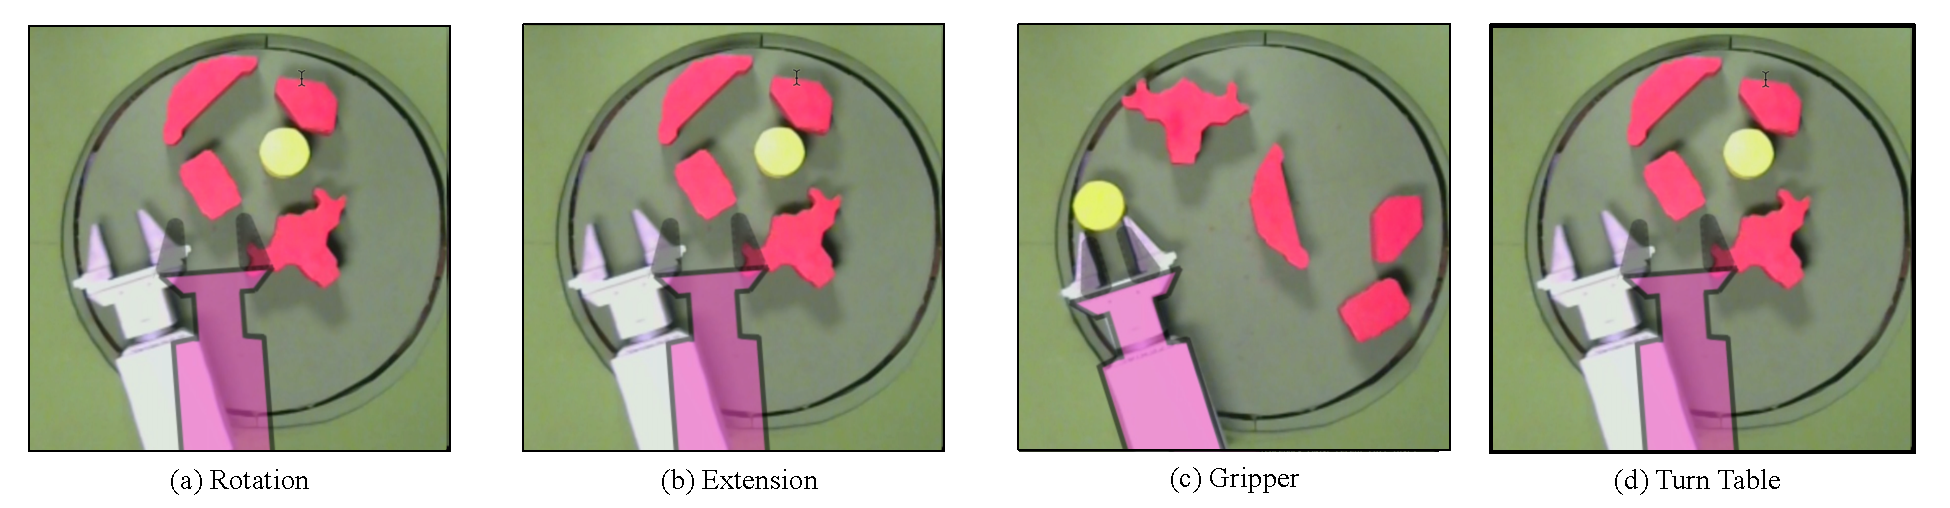
\includegraphics[width=\textwidth]{f_figs/Labeling_GUI.pdf}

\caption{\footnotesize  The interface AMT workers see for providing feedback to the robot for the grasping in clutter task. The pink overlay indicates the desire change in the robot position with respect to the current robot state. Then AMT workers can use their intuition for how objects respond to force to provide examples of how the robot should behave. Each window shows a correction in a degree of freedom a) is the rotation of the robots base b) is extending the robot's arm c) is closing the gripper and d) is rotating the turn table (WILL UPDATE THIS FIGURE)}
\vspace*{-20pt}
\label{fig:overlays}
\end{figure*}





\section{System for Grasping in Clutter Task}
We now detail or experimental system for testing A Gambler's DAgger. First we describe the task itself, then each supervisor in the hierarchy and finally our deep network representation of the policy trained. 

\subsection{Task}
We are interested in training a Zymark robot to perform a grasping in clutter task on image data taken from a Logitech 2000 camera. Examples of images from the camera can be seen in Fig. \ref{fig:teaser}.

The objects in clutter are made Medium Density Fiberboard and each one is on average 4" in diameter. The objects deemed cluttered are painted Red and the goal object is painted yellow. There is an inscribed circle around the work space to keep the robot from pushing the objects outside of the work space. The inscribed circle makes the task more challenging because the robot cannot simply "sweep" the cluttered objects off the table. 

The robot, shown in Fig. \ref{fig:robot}, has a 4 dimensional internal state of base rotation, arm extension, gripper and turn table. The robot is commanded via state position requests, which are tracked by a tuned PID controller. The policy $\pi_\theta$ outputs delta positions that are bounded by $15\deg$ for the gripper and turntable, $1$ cm for the arm extension and $0.5$ cm for the gripper at each time step. There is $T=100$ time steps in a trajectory. 



\subsection{Supervisor Hierarchy}
In this section, we list each supervisor in the order they appear in our hierarchy. The first supervisor is deemed the least expensive. 

\noindent \textbf{Analytical Supervisor} Our first supervisor is a an analytical method that computes the trajectory the robot should move in to reach the goal object, or yellow circle. Our method employs template matching to identify the goal object in the image and the using the forward dynamics of the robot to computes the relative change in direction the robot should apply as an control. The template matching is implemented in OpenCV and uses the normalized cross-correlation filter~\cite{opencv_library}.

In this stage, the analytical supervisors only tries to teach the robot to move towards the goal. Note that the analytical supervisor's advice contains no information about how the cluttered objects will respond to the dynamics applied, which results in sub-optimal polices. However, our analytical supervisor is both computationally and monetarily inexpensive to run which allows us to provide a large number of examples. 


\noindent \textbf{CrowdSourced Supervisor} Our next level of supervisor relies on a crowd source service, called Amazon Mechanical Turk (AMT). Chung et al. demonstrated the reliable data learning from demonstration data could be obtained from an AMT platform. The AMT platform makes readily available thousands of human workers that can perform remedial task for a price range of \$1-0.1\cite{chung2014accelerating}. Thus potentially providing a higher quality supervisor who has an intuition for how the cluttered objects interact with the world, but at a higher cost. 

In order to get quality example from a CrowdSourced Supervisor, we designed an interface shown in Fig. \ref{fig:overlays}. The interface draws a transparent overlay that shows how the robot would respond provided the current control this allows for the AMT worker to see some of the effect of their control. We rely on their natural intuition for how objects to infer how the change in robot position will change the objects.

We also design a tutorial for the work that first has them perform designated motions on a virtual robot and introduces them to a problem. We additionally provide a video of an expert providing corrections on three robot trajectories. 

\begin{figure}[t!]
\centering
\includegraphics[width=\columnwidth, height=4cm]{f_figs/robot.pdf}
\caption{ \footnotesize Shown above is a Zymark robot. The robot consists of an 3DOF arm that lies in a planar workspace and the ability to rotate the turn table. The inscribed circle in the work space prevents the robot from learning the trivial policy of just pushing the objects off the table.}
\vspace*{-10pt}
\label{fig:robot}
\end{figure}


\noindent \textbf{Expert Supervisor} Finally after training with the Analytical and Crowdsourced Supervisor we leverage the Expert supervisor, who is capable of achieving high cumulative reward but is a limited resource, to provide corrections for states that would be non-obvious for someone who doesn't understand the physical limitations of the task. Examples of this could be joint limits of the robot or how some of the objects might respond in more advanced dynamics. \mlnote{After we run the AMT study it will become apparent where an expert is still needed}

It can still be hard for an expert to provide the correct feedback without knowing the magnitude of the controls suggested, so they use the same interface as the CrowdSourced Supervisor. 

\subsection{Deep Neural Network Policy Architecture}
Our policy is represented as deep neural network, which was trained using TensorFlow~\cite{tensorflow2015-whitepaper}. Our network architecture consists of 1 convolutional layer with 5 channels, a fully connected layer with an output of 128 dimensions and a final layer that maps to a four dimensional control signal. We used ReLus to separate the different layers and a final tanh on the output to scale the output between -1 and 1. 

To determine our architecture we created a set of 32,400 different architectures and then performed simulated annealing on the loss function trained after 400 iterations with a batch size of 200. The set of architectures consist of different network architectures as well as different momentum terms, and weight initialization schemes. 

We trained all networks on a dataset of 6K images labeled with the Analytical Supervisor on a Nvidia Tesla K40 GPU, which is able to train each network in an average of 10 minutes.  


\section{Planned Experiments}
All these experiments will be in the grasping clutter domain described above. This section is divided into experiments on reducing supervisor burden via hierarchical supervisor's and testing components on our large scale learning system.  

\subsection{A Gambler's DAgger}

\noindent \textbf{Reducing Supervisor Burden}
In this experiment, we will assign some cost to each supervisor Analytical could be 0.5, Crowdsource 2, and Expert 10 for example. Then compute how many times the expert had to of been queried by using the bootstraped method. We will then do a full DAgger with our experts for comparison to when you don't bootstrap. 

\noindent \textbf{When this Won't Work}
In this experiment, we will look at using two analytical supervisors to try and teach the robot, however they will violate the definition of and not have an overlapping policy (need to think about this a bit). We should see that the supervisor deemed higher in the heirachy has to do roughly if not more queries than without bootstrapping. 

\subsection{System Experiments}

\noindent \textbf{Finding a Neural Network Architecture for Policy Learning}
I want to determine if we can use our analtyical method to find the right architecture by iterating through a dataset. The hypothesis is that you do not need to do roll-outs if you change architecture slightly for better performance (i.e. can I collect a data from rolling out when network and then iterate on that dataset to find the best architecture)

We will see how close a different architectures who received lower training loss on the dataset are to the original trained network in terms of euclidean distance. 

\noindent \textbf{Reliability of Crowdsourced Supervisors}
This experiment is more of a study looking for a few factors, how much data can we get, what is the price point and how lower quality is it to the expert. 

Anca and I discussed an experiment to measure performance against expert. We can then just report our observations in terms of data gathered, time it took and price paid. 


 
\section{Discussions and Future Work}

 \section{Acknowledgments} 
This research was performed in UC Berkeley's Automation Sciences Lab under the UC Berkeley Center for Information Technology in the Interest of Society (CITRIS) "People and Robots" Initiative. This work is supported in part by the U.S. National Science Foundation under Award IIS-1227536, NSF-Graduate Research Fellowship, by the Knut and Alice Wallenberg Foundation and the National Defense Science and Engineering Graduate Fellowship Program. We thank Pieter Abbeel, Sergey Levine and Sanjay Krishnan for insightful feedback. 

  
\bibliographystyle{IEEEtranS}
\bibliography{references}



\end{document}
